\chapter{Arbeidsmetodikk}
\section{Metode}
To arbeidsmetoder ble vurdert i forkant av prosjektet, Scrum og Kanban.

I Scrum begynner man med å definere user stories eller brukerhistorier på formen ``Som (rolle) ønsker jeg (funksjonalitet), sånn at (fordel)''. Disse brukerhistoriene blir gjort om til kort i en product backlog. Videre bestemmer eieren av prosjektet hvilke kort som er viktigst og prioriterer kortene i rekkefølge deretter. Utviklere estimerer hvor lang tid det tar å utføre oppgaven på et kort i timer eller dager. Ut i fra rekkefølgen på kortene og hvor lang tid som er estimert bestemmes hvor mange kort som skal tas med i en iterasjon eller sprint (for eksempel en uke eller to uker). Når en sprint er ferdig skal alle oppgavene være gjort og man skal kunne levere gjeldende funksjonalitet til kunden. En person i teamet får rollen Scrum-master. Scrum-masters oppgave er å legge til rette for at alle får gjort det de skal samt å administrere product backlog'en sammen med produkteieren.

I Kanban har man en product backlog med kort på samme måte som i Scrum, men i steden for å jobbe i sprinter setter man opp en tavle med kolonner som representerer hvilket stadie hver oppgave er i. Eksempler på kolonner kan være:
\begin{itemize}
\item To do
\item In progress
\item In testing
\item Deployed
\end{itemize}
I en kolonne kan det maks være et avtalt antall kort av gangen, for eksempel 4. Dette forhindrer at en oppgave som er påbegynt ikke blir ferdigstilt innenfor rimelig tid.

Gruppen fant sammen med oppdragsgiver ut at Scrum vil føre til i overkant mye prosjektstyring når vi bare er fire stykker i gruppen og har derfor valgt å gå for Kanban. Gruppen mener dette vil gi en smidig utviklingsprosess med god oversikt over hva som må gjøres til en hver tid.

\section{Roller}
For at det skal være klart hvem som har ansvar for hva har gruppen deffinert noen ansvarsområder:
\begin{flushleft}
\renewcommand{\arraystretch}{1.5}
\begin{tabular}[ht]{@{}ll@{}}
\textbf{Gruppeleder} & Espen Bjorøy Zaal \\
\textbf{\LaTeX} & Lukas David Larsed \\
\textbf{Kommunikasjon med oppdragsgiver} & Henrik Fischer Bjelland \\
\textbf{Kommunikasjon med forskningsprosjektsleder} & Espen Bjorøy Zaal \\
\textbf{Versjonskontroll (Git og integrasjon)} & Lukas David Larsed \\
\textbf{Internkommunikasjon (Slack og integrasjon)} & Simen Flatby \\
\end{tabular} 
\end{flushleft}
Ved eventuelle diskusjoner hvor gruppens medlemmer ikke kommer til flerstemt enighet vil gruppeleders stemme telle dobbelt.

\section{Prosjektstyring}
\begin{wrapfigure}{r}{0.5\textwidth}
\vspace{-0.5cm}
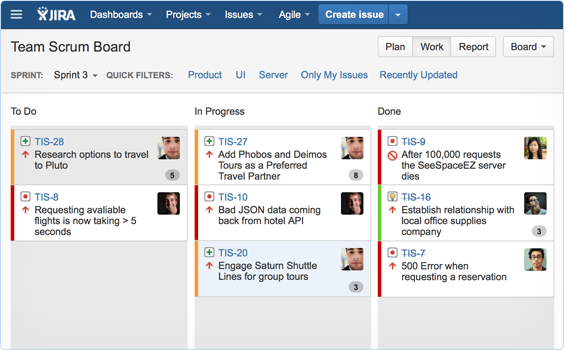
\includegraphics[scale=0.5, keepaspectratio]{./img/arbeidsmetodikk/jira_kanban.png}
\end{wrapfigure}
Til styring av prosjektet har vi valgt å bruke \href{https://www.atlassian.com/software/jira}{Jira}. Jira egner seg godt til bruk med Kanban, og vil hjelpe oss å administrere arbeidsoppgavene våre. Jira har en rekke integrasjoner, og vi vil blant annet benytte oss av GitHub-integrasjonen for å lage koblinger mellom Kanban-kort i Jira og GitHub-issues.
